\chapter{Otvorene inovacije} \label{ch:otvorene_inovacije}

Otvorena inovacija je koncept koji izaziva tradicionalni pristup vertikalnoj
integraciji, gdje interni istraživačko-razvojni (IR\&D) aktivnosti vode internom
razvoju proizvoda koji se potom distribuiraju od strane tvrtke. Umjesto toga,
otvorena inovacija uključuje namjerni unos i izlaz znanja radi ubrzanja interne
inovacije i proširenja tržišta za vanjsko korištenje inovacija, redom
\citep{forbesopeninnovation2011}. Otvorena inovacija je praksa poduzeća i
organizacija da pronalaze ideje iz vanjskih i internih izvora. To znači
dijeljenje znanja i informacija o problemima i traženje rješenja i prijedloga od
ljudi izvan poslovanja \citep{braineetopeninnovation2023}.

\begin{figure}
    \centering
    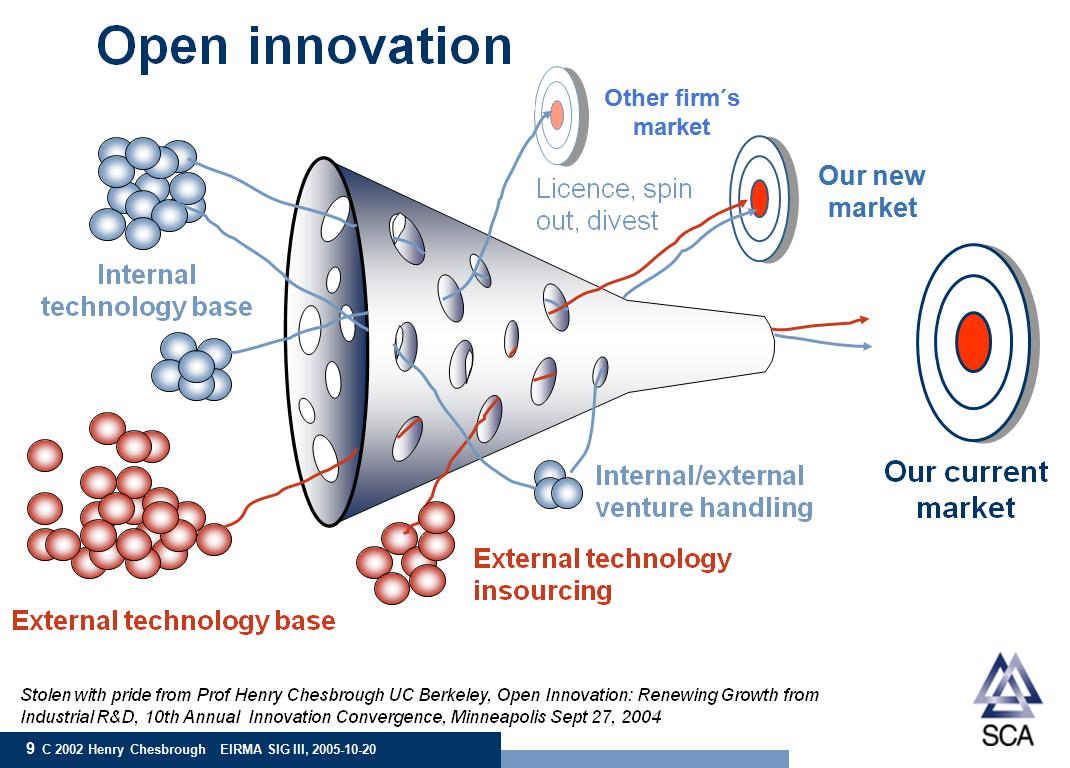
\includegraphics[width=0.8\textwidth]{images/open-innovation11}
    \caption{Prikaz otvorenr inovacije \citep{pakbecopeninnovation2013}.}
    \label{fig:open_innovation}
\end{figure}

Otvorena inovacija se može razumjeti kao antiteza tradicionalnom pristupu
inovaciji. Vanjsko-unutrašnji aspekt se odnosi na unose vanjskih ideja i
tehnologija u vlastiti proces inovacije tvrtke. To je najčešće prepoznata
karakteristika otvorene inovacije. Unutra-vanjski dio je kada neiskorištene ili
nedovoljno iskorištene ideje i tehnologije unutar tvrtke izlaze i inkorporiraju
se u inovacijske procese drugih. Poslovni model je još jedan ključni element
koncepta otvorene inovacije, jer određuje koje ideje i tehnologije treba tražiti
izvana i koje treba pustiti izvan tvrtke \citep{forbesopeninnovation2011}.

Otvorena inovacija nije usmjerena samo na tvrtke; uključuje i kreativne
potrošače i zajednice korisnika-inovatora. Inovacije često dolaze izvana i od
osnivača start-upova, a ne iz postojećih organizacija. Središnja ideja otvorene
inovacije je da u svijetu široko rasprostranjenog znanja tvrtke ne mogu
oslanjati isključivo na vlastita istraživanja, već trebaju kupovati ili
licencirati procese ili izume drugih tvrtki. To se naziva dolaznom otvorenom
inovacijom. Također, interni izumi koji se ne koriste u poslovanju tvrtke
trebaju biti izneseni izvan tvrtke \citep{wikipediaopeninnovation2021}.

Otvorena inovacija nije jednosmjerna ulica. Pozivajući druge da sudjeluju u
generiranju ideja za proizvode i usluge, tvrtke također mogu dijeliti
informacije i stručnost s zajednicama obožavatelja i korisnicima. To stvara
distribuirani, participativniji i decentraliziraniji pristup inovaciji, koji
može otključati mnoge prednosti za poslovanje
\citep{braineetopeninnovation2023}.